\documentclass[fleqn,reqno,10pt]{article}

%========================================
% Packages
%========================================

\usepackage[]{../../helpers/mypackages}
%\usepackage[natbib=true,style=authoryear-comp,backend=bibtex,doi=false,url=false]{biblatex}
%\bibliography{MyRefGlobal}
\bibliography{../../helpers/MyRefGlobal}
\bibliography{paper} 
\usepackage{../../helpers/myenvironments}
\usepackage{../../helpers/mycommands}
\usepackage{todonotes}
\usepackage{subcaption}

\usepackage{a4wide}

%========================================
% Standard Layout
%========================================

% Itemize
\renewcommand{\labelitemi}{\large{$\mathbf{\cdot}$}}    % itemize symbols
\renewcommand{\labelitemii}{\large{$\mathbf{\cdot}$}}
\renewcommand{\labelitemiii}{\large{$\mathbf{\cdot}$}}
\renewcommand{\labelitemiv}{\large{$\mathbf{\cdot}$}}
% Description
\renewcommand{\descriptionlabel}[1]{\hspace\labelsep\textsc{#1}}

% Figure Captions
\usepackage{caption} % use corresponding myfiguresize!
\setlength{\captionmargin}{20pt}
\renewcommand{\captionfont}{\small}
\setlength{\belowcaptionskip}{7pt} % standard is 0pt

%========================================
% Additional layout & commands
%========================================


\renewcommand{\Smixed}{\ensuremath{\mathrm{\mathbf{s}}}}
\renewcommand{\Rmixed}{\ensuremath{\mathrm{\mathbf{r}}}}

% Annotations
\newcommand{\mytodo}[2]{\todo[inline,color=yellow,author=#1]{#2}}
\newcommand{\question}[2]{\todo[inline,color=blue,author=#1]{#2}}
\newcommand{\answer}[2]{\todo[inline,color=green,author=#1]{#2}}

\newcommand{\rd}{\acro{rd}} % replicator dynamic
\newcommand{\rmd}{\acro{rmd}} % replicator mutator dynamic
\newcommand{\rdd}{\acro{rdd}} % replicator diffusion dynamic
\newcommand{\RD}{\ensuremath{\mathrm{RD}}} % replicator dynamic
\newcommand{\RDD}{\ensuremath{\mathrm{RDD}}} % replicator diffusion dynamic
\newcommand{\RMD}{\ensuremath{\mathrm{RMD}}} % replicator mutator
\newcommand{\icid}{\acro{icid}} % imprecise conditional imitation dynamic
\newcommand{\ICID}{\ensuremath{\mathrm{ICID}}} % imprecise conditional imitation dynamic
                                
\newcommand{\Diff}{\ensuremath{\mathrm{D}}} % Difusion 
\newcommand{\Mutate}{\ensuremath{\mathrm{M}}} % Mutation 

\newcommand{\imprecision}{\ensuremath{\alpha}} % imprecision
\newcommand{\toler}{\ensuremath{\beta}} % tolerance
\newcommand{\ns}{\ensuremath{n_s}} % number of states

\newcommand{\similarity}{\ensuremath{\mathrm{Sim}}} % similarity function

\newcommand{\myred}[1]{\textcolor{red}{#1}} 
\renewcommand{\Pr}{\ensuremath{P}} 

\definecolor{Red}{RGB}{178,34,34}
\newcommand{\mf}[1]{\textcolor{Red}{[mf: #1]}} 

% \doublespacing

\title{Vagueness and imprecise imitation in signaling games}
% \author{Michael Franke \and Jos\'e Pedro Correia}
\date{}

\begin{document}

\maketitle

\begin{abstract}
  Signaling games are popular models for studying the evolution of meaning, but typical
  approaches do not incorporate vagueness as a feature of successful signaling.  Complementing
  recent like-minded models, we describe an aggregate population-level dynamic that describes a
  process of imitation of successful behavior under imprecise perception and realization of
  similar stimuli. Applying this new dynamic to a generalization of Lewis' signaling games, we
  show that stochastic imprecision leads to vague, yet by-and-large efficient signal use, and,
  moreover, that it unifies evolutionary outcomes and helps avoid suboptimal
  categorization. The upshot of this is that we see \emph{as-if}-generalization at an aggregate
  level, without agents actually generalizing.
\end{abstract}

\section{Introduction}
\label{sec:introduction}

Many concepts and expressions are vague. A vague category knows clear cases that fall under it,
clear cases that do not, and also so-called borderline cases. Borderline cases do not clearly
apply, nor do they clearly not apply, and there may be differences between borderline cases in
terms of how well they represent the category in question. Vagueness does not seem to
dramatically affect the success of everyday communication, but it is troublesome for some of
the most prominent theories of language and meaning. This is especially so for the
logico-positivist tradition of Frege, Russell, and early Wittgenstein, which is challenged by
the paradoxes vagueness gives rise to.

But there are other intriguing aspects about vagueness. One perplexing issue is how vagueness
could arise and be maintained in the first place. This is an apparent puzzle for functionalist
accounts that maintain that concepts and linguistic meanings evolved driven towards
efficiency. \citet{Lipman2009:Why-is-Language} argues that, in common interest signaling
situations, the existence of unclear borderline cases entails inefficiency of categorization or
communication, or at least no advantage. The challenge is then to explain how vagueness
can persist both: (i) under evolutionary pressure to be optimally discriminative, and (ii)
without undermining the possibility of evolving, learning and communicating with a meaningful
language. A number of authors have consequently tried to explain why vagueness evolved as
something that is itself useful
\citep[e.g.][]{Jaegherde-Jaegher2003:A-Game-Theoreti,Deemter2009:Utility-and-Lan,BlumeBoard2013:Intentional-Vag}.
Others have argued that vagueness is a natural byproduct of limitations in information
processing \citep[e.g.][]{FrankeJager2010:Vagueness-Signa} or of generalization in low-level
learning strategies \citep[e.g.][]{OConnor2013:The-Evolution-o}. This paper contributes to the
latter line of thought.

We believe that vagueness in language and thought may have many reasons, not just one. We focus
here on one \emph{a priori} plausible reason for why vagueness is natural and pervasive. The
idea is that vagueness is, at least in part, due to imprecision in the perception of similar
stimuli and imprecision in the realization of similar responses. On this view, vagueness in
language may be seen as a necessary sub-optimality due to limitations in another domain of
cognition, first and foremost perception. It could then be speculated that the whole system,
perception and language together, may be an almost optimal adaptation in a larger frame
of reference, e.g., if we take into account the metabolic costs for increased perceptual
accuracy. We will not engage in such speculation here. Rather we will explore the consequences
of perceptual limitations on processes of meaning evolution in a suitable formal framework. In
other words, in order to address Lipman's challenge seriously, and not just hand-wave it away
by appeal to the naturalness of vagueness, it needs to be spelled out how exactly confusability
of stimuli could come into play in a process of meaning evolution and how it could lead to
vague but by-and-large informative signal meaning. The formal model that this paper introduces
does exactly that. But it also does more. We find that confusability of stimuli can regularize
and systematize evolving meaning. This suggests a possibly advantageous side-effect that a
natural cause of vagueness may have and that might compensate some of the disadvantages that
vagueness may have for communicative efficiency \citep[c.f.][]{OConnor2013:The-Evolution-o}.

% The replicator mutator dynamic is neat because it keeps the effects of fitness-based selection
% (replication) and transmission biases (mutation) nicely apart. This is possible because it
% adheres to a picture of (asexual) biological reproduction: the number of children a (single)
% parent has is higher, the higher the communicative success of the parent's language; all
% children of this parent will learn from this parent alone, but may make mistakes during
% language acquisition.

The next section introduces the background against which the work presented here can be
appreciated. Section~\ref{sec:repl-diff-dynam} introduces a generalization of the replicator
dynamic which is derived from the idea that agents imitate other agents' behavior while
possibly confusing similar states. This imprecise imitation dynamic is explored in
Section~\ref{sec:exploring-rdd}. Section~\ref{sec:discussion} reflects and compares our
approach to others. Appendix~\ref{sec:formal-stuff} provides formal detail.

\section{Background}
\label{sec:background}

% The view that vagueness is a natural concomitant of cognitive
% limitations of language users has been formalized in a number of ways,
% using evolutionary game theory and certain generalizations of Lewis'
% signaling games \citep{Lewis_1969:Convention}, so called
% \emph{similarity-maximizing games}, or \emph{sim-max games}, for short
% \citep{Jager2007:The-Evolution-o,JagerRooijvan-Rooij2007:Language-Struct}.
% %\citep{FrankeJager2010:Vagueness-Signa,OConnor2013:Evolving-Percep,OConnor2013:The-Evolution-o}.
% Our contribution is best seen in relation to these accounts, as it also
% relies on sim-max games. Let's introduce these first, and then zoom in
% on the problem of vagueness.

\subsection{Sim-max games \& conceptual spaces}

Signaling games, as introduced by \citet{Lewis_1969:Convention}, have
a sender and a receiver. The sender knows the true state of the world,
but the receiver does not. The sender can select a signal, or message,
to reveal to the receiver, who then chooses an act. In Lewis' games,
if the receiver chooses the act that corresponds to the actual state,
the play is a success, otherwise a failure. Certain regular
combinations of sender signaling and receiver reaction make messages
meaningful, in the sense that their use is correlated systematically
to certain states or acts. To investigate the conditions under which
such meaning-generating behavior can evolve is a highly interesting
topic that we are only beginning to fully understand
\citep[e.g.][]{Warneryd1993:Cheap-Talk-Coor,BlumeKim1993:Evolutionary-St,Huttegger2007:Evolution-and-t,Pawlowitsch2008:Why-Evolution-d,Barrett2009:The-Evolution-o,HutteggerSkyrms2010:Evolutionary-Dy,Skyrms2010:Signals}.

Similarity-maximizing (short: sim-max) games are a variation of Lewis' games where the
receiver's actions are equated with the state space (one can think of the actions as choosing
states) and different states are allowed to be more or less similar to one another. While
Lewis' games treated communicative success as a matter of black and white, sim-max games allow
for shades of gray: the more similar the receiver's interpretation is to the actual state, the
better. Signaling games with utility-relevant similarities in the state space are fairly
standard in economics
\citep[e.g.][]{Spence1973:Job-market-sign,CrawfordSobel1982:Strategic-Infor}, but have received
particular attention in a more philosophical context for reasons that will become clear
presently.

Formally, a sim-max game consists of a set of states $\States$, a set of messages $\Messgs$
typically with much fewer messages than states, a probability distribution
$\Pr \in \Delta(\States)$ such that $\Pr(\state)$ gives the probability that state $\state$
occurs, a similarity metric\footnote{A metric is a function of distance between any two points
  in a given space. It should satisfy certain axioms that ensure behavior that one would
  intuitively expect from the words ``similarity'' and ``distance'' alone, but these details do
  not matter for the purposes of this paper. The assumption that state similarity forms a
  metric is conceptually loaded, but we follow the literature here and conceive of it as a
  first and pragmatic simplification, possibly to be dispensed with later.}
  % : similarity should always be non-negative, zero only for the distance
  % between an element and itself, symmetric, and satisfy the triangle inequality that
  % $\similarity(x,z) \le \similarity(x,y) + \similarity(y,z)$
on states $\similarity \mycolon \States \times \States \rightarrow \mathds{R}$ such that
$\similarity(\mystate{1}, \mystate{2})$ is the (physical) similarity between $\mystate{1}$ and
$\mystate{2}$, and a utility function
$\Utils \mycolon \States \times \States \rightarrow \mathds{R}$ such that
$\Utils(\mystate{1}, \mystate{2})$ is the payoff for sender and receiver for a play with actual
state $\mystate{1}$ and receiver interpretation $\mystate{2}$. We identify the receiver's acts
with the states of the world, so that the game is one of guessing the actual state, so to
speak. For the modeling purposes of this paper, we make the simplifying assumption that
$\States$ is a set of points in Euclidean space, whose closeness to each other tracks physical
similarity. Perceived similarity, where it is necessary, would be a monotonic function of
physical similarity. Likewise, the utility function should be a monotonically increasing
function of physical similarity.\footnote{Section~\ref{sec:setting-stage} motivates particular
  choices of similarity and utility functions that we will explore in more detail.}
Non-probabilistic sender behavior can be represented by a pure strategy
$\Spure \in \Messgs^\States$, which deterministically defines which message would be used for
each state. Similarly, a pure receiver strategy is a function $\Rpure \in \States^\Messgs$.


\citet{JagerMetzger2011:Voronoi-Languag} showed that the evolutionarily stable states of sim-max games with infinitely many states in $n$-dimensional Euclidean space $\States \subseteq \mathds{R}^n$ and a quadratic loss function for utilities $\Utils(\mystate{1}, \mystate{2}) = - (\mystate{1} - \mystate{2})^2$ are remarkably systematic: the evolutionarily stable states are demonstrably so-called Voronoi languages.
Roughly put, a Voronoi
language is a pair of sender and receiver strategies, such that the sender strategy partitions
the state space into convex categories, while the receiver's interpretations are the central
spots in each category. A subset $X$ of $\mathds{R}^n$ is convex if, informally put, all points
in $X$ are connected via a straight line that lies entirely in $X$; $X$ has no gaps or
dents. For example, if \States is the unit interval and all states are equiprobable, a Voronoi
language with two messages could have the sender use one message exclusively for all points in
the lower half of the unit interval and another for all points in the upper half; the
receiver's interpretations of messages are the central points, .25 and .75, in the respective
intervals.  See Figure~\ref{fig:Voronoi-language-example} for an illustration.

\begin{figure}
  \centering

  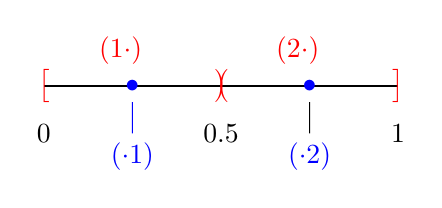
\begin{tikzpicture}[scale=3]

        \begin{scope}

          \draw[-,thick] (0,0) -- (1.5,0);

          \draw (0,0) node {\color{red}{\big{[}}};

          \draw (.75,0) node {\color{red}{\big{)}}};

          \draw (.76,0) node {\color{red}{\big{(}}};

          \draw (1.5,0) node {\color{red}{\big{]}}};

            \draw (.325,.15) node
            {\color{red}{$\Spure(\mymessg{1}  \probbar \cdot)$}};

            \draw (1.075,.15) node
            {\color{red}{$\Spure(\mymessg{2} \probbar \cdot)$}};

            \node at (.375,0) (node1) {\color{blue}{$\bullet$}};

            \node at (.375,-.3) (label1)
            {\color{blue}{${\Rpure}(\cdot \probbar \mymessg{1})$}};

            \draw[-,color=blue] (node1) -- (label1);

            \node at (1.125,0) (node2) {\color{blue}{$\bullet$}};

            \node at (1.125,-.3) (label2)
            {\color{blue}{${\Rpure}(\cdot \probbar \mymessg{2})$}};

            \draw[-] (node2) -- (label2);

            \draw (0,-.2) node {$0$};

            \draw (.75,-.2) node {$0.5$};

            \draw (1.5,-.2) node {$1$};

          \end{scope}
 
         \end{tikzpicture}

        \caption{Example of a Voronoi language on $\States = [0,1]$. The pure sender strategy
          $\Spure$ uses one signal for the lower half, and another for the upper half of the
          unit interval. The pure receiver strategy $\Rpure$ selects the central elements in
          the respective intervals. See \citet{JagerMetzger2011:Voronoi-Languag} for further
          details.}
  \label{fig:Voronoi-language-example}
\end{figure}


It is intuitive to think that linguistic and conceptual categories are orderly in such a
manner.  For example, if you consider two people `tall', one with a height of 2m and another with a
height of 2.2m, it would be difficult to defend not considering a person with a height
of 2.1m `tall' as well. Another example where this intuition is additionally supported by empirical data is that of color categorization. The World Color Survey
project~\citep{CookKay2005:The-World-Color,WCS} collected color naming data for 110 unwritten
languages of 45 language families.  For the great majority of these languages a pattern can be
observed: basic color terms are by and large convex~\citep{Regier07,Jager2010}. It
is premature to argue that these observations can be extended to \emph{all} cases of
categorization. However, for the cases where it does apply, the result of
\citet{JagerMetzger2011:Voronoi-Languag} is interesting because it demonstrates that signaling
can impose this kind of orderly categories on a metric space without that being the ulterior
purpose of it all.%
\footnote{For the concrete case of color categorization, see also
  \citet{JagerRooijvan-Rooij2007:Language-Struct} and \citet{Correia2015}}
Finally, these considerations are in line with a prominent
school of thought in comparative linguistics which also assumes that more abstract conceptual domains
(e.g., spatial-topological relations, temporal reference, or the meanings expressible by
indefinite pronouns) are preferably carved up by the languages of the world in such a way
that meanings are connected regions on a so-called \emph{semantic map}
\citep[e.g.][]{Croft2003:Typology-and-Un,Haspelmath2003:The-geometry-of,LevinsonMeira2003:Natural-concept}.

There are at least two potential ways of interpreting the signaling setup.
Sender and receiver can be distinct
entities, whose purpose is to communicate effectively about the actual
state. In that case, evolving Voronoi languages would explain why
\emph{linguistic categories} are well-behaved and orderly in the way
they appear to be. More abstractly, sender and receiver can also be
thought of as distinct modules in a single system, where the first
module must discretize the information it is fed by selecting a small
sample of, suggestively, category labels. These are passed to a second
module that tries to decode the original information. In this case,
evolving Voronoi languages would explain why \emph{conceptual
  categories} are well-behaved and orderly in the way that they appear
to be.
Seen in this light, sim-max games may provide a foundation to approaches in cognitive semantics
that rely on the notion of conceptual spaces.
\citet[][70--77]{Gardenfors2000:Conceptual-Spac}, for example, has prominently argued that
natural categories are convex regions in conceptual space. If the conceptual space has a
suitable metric, convex categories can be derived from a set of prototypes. The category
corresponding to prototype $p$ is the set of points that are more similar to $p$ than to any
other. In this way, \citeauthor{Gardenfors2000:Conceptual-Spac} argues, an efficient categorization
system can be obtained: storing the prototypes lets us recover the categories without having to
store each category's extension. However, what is left unexplained is where the prototypes
come from, and why we would not see just any distribution of prototypes as an equally efficient
classification system. This is where sim-max games can contribute a principled approach to
deriving, in an independent way, not only convex categories but also prototypical exemplars
belonging to them.  These ideas, and more, are developed further by
\citet{Jager2007:The-Evolution-o,JagerRooijvan-Rooij2007:Language-Struct,JagerMetzger2011:Voronoi-Languag,OConnor2014-OCOEPC},
among others.

\subsection{Vagueness in sim-max games and conceptual spaces}

This outline of an approach to categorization using sim-max games
leaves many problems unaddressed. One of them is that natural
categories for continuously variable stimuli usually do not have
unique, point-valued prototypes and clear category boundaries. We
would like to account for the possibility of such vagueness, in
particular: (i) clear positive examples of a vague category should
show a gradient transition to clear negative examples;
(ii) prototypes should likewise be gradient regions, peaking at the
center of the vague category they represent.

\citet{DouvenDecock2011:Vagueness:-A-Co} show that
\citeauthor{Gardenfors2000:Conceptual-Spac}'s conceptual spaces
approach can be extended to account for the existence of borderline
cases. From the assumption that prototypes are extended, yet convex
regions in conceptual space, a construction algorithm is available
that yields ``collated Voronoi diagrams'' with thick boundaries
representing borderline
regions. \citet{DecockDouven2012:What-is-Graded-} show further how it
is possible to arrive at a gradient transition between categories, by
weighing in the distance of different borderline cases to various
prototypical regions. This accounts for the first of the two
desiderata mentioned above, but still assumes that crisp prototype
regions must be given.

Alternative approaches are taken by, for example, \citet{FrankeJager2010:Vagueness-Signa} and
\citet{OConnor2013:The-Evolution-o}, who show different ways how the above desiderata can be
met by evolving strategies in sim-max games. To illustrate what vague signaling would look
like, let us briefly consider a sim-max game with six equiprobable states and two messages and
what its equilibria would be like \citep[see][for a more thorough discussion of equilibria of
sim-max games]{Jager2007:The-Evolution-o,OConnor2013:The-Evolution-o}. We assume that utilities
are linearly decreasing with decreasing similarity. Figure~\ref{fig:EquilibriaVagueness} shows
three pairs of sender and receiver strategies. States are arranged according to their
similarity: the closer they are to each other, the more similar they are. The pair in
Figure~\ref{fig:ineffNonEq} is not an equilibrium, because the sender's non-convex use of
signals is suboptimal given the receiver's behavior. Namely, if \mymessg{1} is interpreted as
\mystate{2} and \mymessg{2} as \mystate{4}, then the sender would get a higher payoff from
sending \mymessg{1} in \mystate{3} than from sending \mymessg{2}, because (by assumption)
\mystate{3} is more similar to \mystate{2} than \mystate{5} is. In contrast,
Figure~\ref{fig:efficientEq} shows a maximally efficient equilibrium. This is a partial pooling
equilibrium in the sense that the speaker uses the same message for several states. Partial
pooling equilibria can be less inefficient than other non-pooling equilibria, if there are
enough messages. The strategy pair of Figure~\ref{fig:efficientEq} is maximally efficient for
the two-message case. So, while partial pooling may entail inefficiency in some sense, and
while partial pooling can hamper the evolution of maximally efficient signal use
\citep[e.g.][]{Hutteger:2007_Evol_Indicatives_Imperatives,Pawlowitsch2008:Why-Evolution-d,HutteggerSkyrms2010:Evolutionary-Dy},
this is orthogonal to our concerns about vagueness. A regular and natural yet vague signal use
would look like the pair in Figure~\ref{fig:vagueUse}. This is not an equilibrium, but it gets
close, so to speak. It shows smooth transitions across similar states at the boundaries of
categories and across acts around the most prototypical instances (as indicated by decreasing
thickness of arrows in Figure~\ref{fig:vagueUse}).

\begin{figure}
  \centering
  
  \begin{subfigure}[]{0.475\textwidth}
    \centering
    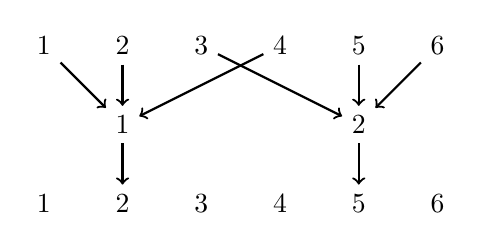
\begin{tikzpicture}

      \draw[] (0,2) node (t1) {$\mystate{1}$};

      \draw[] (1,2) node (t2) {$\mystate{2}$};

      \draw[] (2,2) node (t3) {$\mystate{3}$};

      \draw[] (3,2) node (t4) {$\mystate{4}$};

      \draw[] (4,2) node (t5) {$\mystate{5}$};

      \draw[] (5,2) node (t6) {$\mystate{6}$};


      \draw[] (1,1) node (m1) {$\mymessg{1}$};

      \draw[] (4,1) node (m2) {$\mymessg{2}$};



      \draw[] (0,0) node (a1) {$\mystate{1}$};

      \draw[] (1,0) node (a2) {$\mystate{2}$};

      \draw[] (2,0) node (a3) {$\mystate{3}$};

      \draw[] (3,0) node (a4) {$\mystate{4}$};

      \draw[] (4,0) node (a5) {$\mystate{5}$};

      \draw[] (5,0) node (a6) {$\mystate{6}$};

      % arrows
  
      \draw[->, thick] (t1) -- (m1);

      \draw[->, thick] (t2) -- (m1);

      \draw[->, thick] (t3) -- (m2);

      \draw[->, thick] (t4) -- (m1);

      \draw[->, thick] (t5) -- (m2);

      \draw[->, thick] (t6) -- (m2);

      \draw[->, thick] (m1) -- (a2);

      \draw[->, thick] (m2) -- (a5);
  
    \end{tikzpicture}

    \caption{inefficient, non-convex, non-equilibrium}
    \label{fig:ineffNonEq}
  \end{subfigure}
  \hfill
  \begin{subfigure}[]{0.475\textwidth}
    \centering

    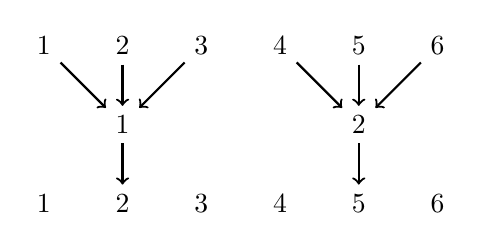
\begin{tikzpicture}

      \draw[] (0,2) node (t1) {$\mystate{1}$};

      \draw[] (1,2) node (t2) {$\mystate{2}$};

      \draw[] (2,2) node (t3) {$\mystate{3}$};

      \draw[] (3,2) node (t4) {$\mystate{4}$};

      \draw[] (4,2) node (t5) {$\mystate{5}$};

      \draw[] (5,2) node (t6) {$\mystate{6}$};


      \draw[] (1,1) node (m1) {$\mymessg{1}$};

      \draw[] (4,1) node (m2) {$\mymessg{2}$};



      \draw[] (0,0) node (a1) {$\mystate{1}$};

      \draw[] (1,0) node (a2) {$\mystate{2}$};

      \draw[] (2,0) node (a3) {$\mystate{3}$};

      \draw[] (3,0) node (a4) {$\mystate{4}$};

      \draw[] (4,0) node (a5) {$\mystate{5}$};

      \draw[] (5,0) node (a6) {$\mystate{6}$};

      % arrows
  
      \draw[->, thick] (t1) -- (m1);

      \draw[->, thick] (t2) -- (m1);

      \draw[->, thick] (t3) -- (m1);

      \draw[->, thick] (t4) -- (m2);

      \draw[->, thick] (t5) -- (m2);

      \draw[->, thick] (t6) -- (m2);

      \draw[->, thick] (m1) -- (a2);

      \draw[->, thick] (m2) -- (a5);
  
    \end{tikzpicture}

    \caption{maximally efficient equilibrium, partial pooling}
    \label{fig:efficientEq}
  \end{subfigure}

\begin{subfigure}[]{0.475\textwidth}
    \centering

    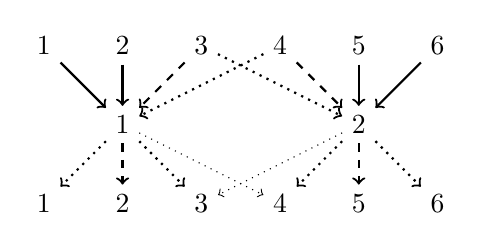
\begin{tikzpicture}

      \draw[] (0,2) node (t1) {$\mystate{1}$};

      \draw[] (1,2) node (t2) {$\mystate{2}$};

      \draw[] (2,2) node (t3) {$\mystate{3}$};

      \draw[] (3,2) node (t4) {$\mystate{4}$};

      \draw[] (4,2) node (t5) {$\mystate{5}$};

      \draw[] (5,2) node (t6) {$\mystate{6}$};


      \draw[] (1,1) node (m1) {$\mymessg{1}$};

      \draw[] (4,1) node (m2) {$\mymessg{2}$};



      \draw[] (0,0) node (a1) {$\mystate{1}$};

      \draw[] (1,0) node (a2) {$\mystate{2}$};

      \draw[] (2,0) node (a3) {$\mystate{3}$};

      \draw[] (3,0) node (a4) {$\mystate{4}$};

      \draw[] (4,0) node (a5) {$\mystate{5}$};

      \draw[] (5,0) node (a6) {$\mystate{6}$};

      % arrows
  
      \draw[->, thick] (t1) -- (m1);

      \draw[->, thick] (t2) -- (m1);

      \draw[->, thick, dashed] (t3) -- (m1);

      \draw[->, thick, dotted] (t3) -- (m2);

      \draw[->, thick, dotted] (t4) -- (m1);

      \draw[->, thick, dashed] (t4) -- (m2);

      \draw[->, thick] (t5) -- (m2);

      \draw[->, thick] (t6) -- (m2);

      \draw[->, thick, dotted] (m1) -- (a1);

      \draw[->, thick, dashed] (m1) -- (a2);

      \draw[->, thick, dotted] (m1) -- (a3);

      \draw[->, dotted] (m1) -- (a4);

      \draw[->, dotted] (m2) -- (a3);

      \draw[->, thick, dotted] (m2) -- (a4);

      \draw[->, thick, dashed] (m2) -- (a5);

      \draw[->, thick, dotted] (m2) -- (a6);
  
    \end{tikzpicture}

    \caption{almost efficient, probabilistic, intuitively vague}
    \label{fig:vagueUse}
  \end{subfigure}


  \caption{Examples of strategy pairs in sim-max games. Sender strategies map states onto
    messages (top two rows); receiver strategies map messages onto states (bottom two rows). In
    Figure~\ref{fig:EquilibriaVagueness}, the thickness of arrows indicates the probability of
    a choice in a probabilistic strategy.}
  \label{fig:EquilibriaVagueness}
\end{figure}

\subsection{Vagueness, functional pressure \& transmission biases}
\label{sec:vagu-funct-press}

The approach we take here is similar in spirit to that of
\citet{FrankeJager2010:Vagueness-Signa} and \citet{OConnor2013:The-Evolution-o}, but different
in relevant detail. A more in-depth comparison is deferred until
Section~\ref{sec:discussion}. Let us first motivate our approach here, and spell it out in more
detail in the following section.

Our conceptual starting point is the widely shared conviction that language is shaped by at
least two forces, which may, on occasion, pull in opposite direction. On the one hand, there is
functional pressure towards efficient communication. On the other hand, there is systematic
error, noise or imprecision in the transmission of linguistic behavior, knowledge or traits. As
an example for the latter, consider a child learning syntactic rules from a parent
generation. The child must infer these unobservable rules from observable speech. Inductive
biases may influence which syntactic rules are likely to be inferred from (finite) parental
input. Over the course of many generations, the effects of such biases can, in a manner of
speaking, ``accumulate'' and lead to surprising results, such as the evolution of compositional
form-meaning mappings or the use of regular recursive syntactic structure. This can happen when
the effects of tranmission biases are isolated, as in iterated learning models
\citep{KirbyHurford2002:The-Emergence-o,SmithKirby2003:Iterated-Learni,GriffithsKalish2007:Language-Evolut,KirbyGriffith2014:Iterated-Learni},
or when they interact with functional pressure towards efficient communication, e.g., as
formalized in the replicator mutator dynamic
\citep[e.g.][]{NowakPlotkin2000:The-Evolution-o,NowakKomarova2001:Evolution-of-Un}.

The emphasis of previous models that studied the effects of transmission infidelity on the
evolution of language has been on inductive biases and the systematicity, compression and
regularization that they can introduce. Here, we would like to show that transmission noise of
a different kind can lead to regularization as well and also give rise to vague meaning. We
find that shared perceptual biases that perturb the transmission of successful signaling
behavior can regularize, facilitate and accelerate the evolution of meaning conventions, albeit
at the cost of vagueness. Concretely, we formalize the expected change in the behavior of a
population of agents that try to imitate other agents' signaling behavior. We assume, however,
that both realization of behavior, as well as observability of others' behavior, is
systematically perturbed by noise. The resulting population-level dynamic generalizes the
replicator dynamic \citep{TaylorJonker1978:Evolutionary-St} in its interpretation as a cultural
evolutionary dynamic based on imitation
\citep[e.g.][]{Helbing1996:A-Stochastic-Be,Schlag1998:Why-Imitate-and}. The inclusion of
confusability of stimuli does not undermine the possibility of evolving communicative signaling
behavior. Instead, it leads to the evolution of vague meanings. It moreover accelerates the
emergence of communicative signaling because it unifies and regularizes evolutionary outcomes,
making it appear as if agents were applying inductive biases or generalizing over partial
observations, when in truth this is the sole effect of confusion of similar stimuli.



%%%%%%%%%%%%%%%%%%%%%%%%%%%%%%%%%%%%%%%%%%%%%%%%%%
%%%%%%%%%%%%%%%%%%%%%%%%%%%%%%%%%%%%%%%%%%%%%%%%%%

\section{Imprecise imitation}
\label{sec:repl-diff-dynam}

Signaling agents can adapt their dispositions to act, given some feedback about their past
success, in multiple ways. Usually, we would assume that changes in behavior should, at least
on average, lean towards increasing chances of communicative success. Such behavioral
adaptations can be described at different levels of abstraction. At the level of individual
agents, we can picture a more or less idealized process of how each agent adapts dispositions
for future actions based on various pieces of information available to the agent. More
abstractly, at the level of a population of agents, we can describe how average behavioral
dispositions will evolve. The population-level perspective abstracts over small stochastic
fluctuations and zooms in on the general tendency or direction of evolution that ensues from
behavior at the agent-level.

To better understand the interaction of confusability of stimuli and selective pressure towards
successful communication, we look at a population-level dynamic that describes the most likely
evolutionary path of a population of signaling agents who imitate other agents' behavior but
are liable to confuse states for one another. In the special limiting case where state
confusability vanishes, the process is just the well-known replicator dynamic
\citep{TaylorJonker1978:Evolutionary-St}, which should therefore be briefly reviewed first.


\subsection{Replicator dynamic in behavioral strategies}
\label{sec:repl-dynam-behav}

Fix a sim-max game with finite states $\States$ and messages $\Messgs$. As usual, we assume
that the receiver chooses states in $\States$ in response to messages. Let
$\Pr(\cdot) \in \Delta(\States)$ be the prior distribution over states and
$\Util \mycolon \States \times \States \rightarrow \mathds{R}$ the utility function shared by
senders and receivers in the population. A \emph{behavioral strategy} is a function that maps
an agent's choice points to a probability distribution over available
choices.\footnote{\label{fn:mixedStrats}Our focus is on behavioral strategies, not \emph{mixed
    strategies}, i.e., probability distributions over functions from each choice point to an
  act, such as $s \in \Delta(\Messgs^{\States})$.  Dynamics on behavioral strategies assume
  that agents can adapt their behavior locally, i.e., independently at each choice point. Our
  focus on behavioral strategies greatly reduces the complexity of the dynamic and simplifies
  numerical simulations. But it also seems the more plausible choice for imitation-based update
  protocols of the kind we consider here: agents only observe how, on some occasion, some other
  agent behaved in \emph{one} particular situation, not how that agent would behave in
  \emph{all} relevant choice situations; they imitate the use of a single word, so to speak,
  not a whole lexicon. (See \citet{Cressman2003:Evolutionary-Dy} for more on the difference
  between dynamics on mixed or behavioral strategies.) It is in this respect that the cultural
  evolutionary dynamic introduced here differs most visibly from the replicator mutator dynamic
  \citep[e.g.][]{NowakPlotkin2000:The-Evolution-o,NowakKomarova2001:Evolution-of-Un}, which
  operates on mixed strategies and is motivated by assumptions of (asexual) biological
  inheritance with transmission infidelity.} The sender's behavioral strategies are
functions $\Sstrat \in \Delta(\Messgs)^\States$, thus mapping each state $\state \in \States$
to a probability of each message $\messg \in \Messgs$ being sent in $\state$; the receiver's
are functions $\Rstrat \in \Delta(\States)^\Messgs$, thus mapping each message
$\messg \in \Messgs$ to a probability of each interpretation $\state \in \States$ being chosen
in response to $\messg$. Although behavioral strategies are probabilistic, evolutionary
modeling usually imagines that every individual agent has a non-probabilistic
strategy. Behavioral strategies then capture average population behavior. Assuming a virtually
infinite population, the number $\Sstrat(\messg \probbar \state)$, for instance, is then the
probability that a randomly sampled sender would send message $\messg$ if the actual state was
$\state$. Similarly, $\Rstrat(\state \probbar \messg)$ is then the probability with which a
randomly sampled receiver interprets $\messg$ as $\state$. A play of a single evolutionary game
with behavioral strategies is illustrated in Figure~\ref{fig:sim-max-illustration}.

\begin{figure}
  \centering

  \begin{tikzpicture}[->,auto,semithick,>=stealth',every label/.style={gray},node distance=0.9cm]

  \node (1) {};
  \node (2) [right=of 1,label=below:$\Pr(\mystate{1})$] {$\mystate{1} \in \States$};
  \node (3) [right=of 2,label=below:$\Sstrat(\messg \probbar \mystate{1})$] {$\messg \in \Messgs$};
  \node (4) [right=of 3,label=below:$\Rstrat(\mystate{2} \probbar \messg)$] {$\mystate{2} \in \States$};

  \path
    (1) edge node {N} (2)
    (2) edge node {S} (3)
    (3) edge node {R} (4);

  \end{tikzpicture}

  \caption{A round of play in a sim-max game with behavioral strategies: Nature (N) chooses a
    state $\mystate{1}$ with probability $\Pr(\mystate{1})$; a random sender (S) selects a
    message $\messg$ with probability $\Sstrat(\messg \probbar \mystate{1})$; a random receiver
    (R) selects a state $\mystate{2}$ with probability $\Rstrat(\mystate{2} \probbar \messg)$.
    Payoff for both sender and receiver is given by $\Utils(\mystate{1}, \mystate{2})$.}
   %which is typically proportional to state similarity $\similarity(\mystate{1}, \mystate{2})$.}
  \label{fig:sim-max-illustration}
\end{figure}

The \emph{expected utility} of choices at each choice point is:\footnote{The notation
  $\propto$, for ``proportional to'', that is used here and hereafter means that the right-hand
  side might still need to be normalized so as to have probabilities sum to one. In general,
  writing $P(x) \propto f(x)$ for any function $f \mycolon X \rightarrow \mathds{R}$ is
  shorthand for $P(x) = \frac{f(x)}{\sum_{x' \in X} f(x')}$. }
\begin{align*}
  \EU(\messg, \state, \Rstrat) & = \sum_{\state \in \States}
  \Rstrat(\state' \probbar \messg) \myts U(\state, \state') \\
  \EU(\state', \messg, \Sstrat) & = \sum_{\state \in
    \States} P(\state \probbar \messg)  \myts
  U(\state, \state')\,, \text{\ \  where } &
P(\state \probbar \messg) & \propto \Pr(\state) \myts \Sstrat(\messg \probbar \state) \,.
\end{align*}
Expected utilities are sums, over all possible concrete outcomes, of the utilities of these
outcomes, weighted by how likely they occur. For instance, the expected utility for the sender
of choosing message $\messg$, given state $\state$ and a receiver strategy $\Rstrat$ is the
sum, for each interpretation $\state'$, of the probability that some random receiver will
choose $\state'$ given $\messg$ times the actual utility of pair $\state$ and
$\state'$.

The discrete-time replicator dynamic tracks changes in frequency of choices in the population
as proportional to their expected utilities
\citep[e.g.][]{HofbauerSigmund1998:Evolutionary-Ga}:\footnote{The formulation given in
  Equation~(\ref{eq:RDDiscrete}) is adequate only for cases like the one we will be looking at
  in Section~\ref{sec:exploring-rdd}, where utilities are always non-negative and expected
  utilities are always positive.}
\begin{align}
  \label{eq:RDDiscrete}
  \Sstrat'(\messg \probbar \state) & \propto \Sstrat(\messg \probbar \state) \myts
    \EU(\messg, \state,\Rstrat)\,, & \Rstrat'(\state \probbar \messg) & \propto \Rstrat(\state \probbar \messg) \myts
    \EU(\state, \messg,\Sstrat)\,.   
\end{align}
For a given choice point, say a state $\state$, the probability of seeing $\messg$ played by an
average agent in the population \emph{after} the update is proportional to the probability of
seeing it \emph{before} the update, which is $\Sstrat(\messg \probbar \state)$, times the
expected utility of $\messg$ at state $\state$. Intuitively put, frequencies of choices change
by a gradient of current frequency and a measure of how good they are.

The replicator dynamic is an abstract population-level dynamic that describes the mean expected
change of behavioral dispositions in a population of signalers. There are several ways of
deriving the replicator dynamic from agent-level processes of behavioral adaptation. We focus
here on one of the simplest: \emph{imitation of success}
\citep[see][]{Sandholm2010:Population-Game}. The intuitive idea is the following (see
Appendix~\ref{sec:cond-imit-succ} for a derivation of the standard replicator dynamic from this
update scheme).  Every now and then a random agent gets a chance to alter his behavior for one
of his choice points. Say, this is a sender who gets to ``reconsider'' his choice of message
for state $\state$. The revising agent then observes what some random agent does at $\state$,
say $\messg$, and will henceforth play $\messg$ in $\state$ with a probability given by the
expected utility of $\messg$ for state $\state$.

\subsection{Noise perturbed conditional imitation}
\label{sec:noisy-repl-dynam}

Imitation of success, as described above, presupposes that agents make no mistakes when
observing states, or choosing interpretations. This may not always be an appropriate
assumption, especially when some states can be perceptually similar and therefore likely to be
confused for one another.
Human performance in these situations has been studied by a number of authors in experimental psychology. %~\citep{takane_structures_1992}.
In a stimulus identification experiment~\citep{luce_detection_1963}, subjects are presented in each trial with a stimulus to be identified out of a fixed set.
The more similar the stimuli are to each other, the larger the number of errors subjects make.
For example, in Robert Nosofsky's experiments~\citep{Nosofsky1986:Attention-Simil}, stimuli consisted of 16 semicircles with a radial line from the center to the rim, varying in size (radius of 0.478, 0.500, 0.522, or 0.544 cm) and angle of the line (50º, 53º, 56º, or 59º).
In over 9000 trials, the two subjects identified the stimulus correctly only approximately 44\% and 35\% of the time.
Similar experiments have been conducted with other identification tasks, for example, for frequency and intensity of tones, taste, hue of colors, and magnitude of lines and areas~\citep{donkin_why_2015}.
The empirical data confirms not only the pervasiveness of variation in the subjects' ability to correctly identify stimuli, but also the relation between similarity and likelihood of stimulus confusion, and further suggests that the phenomenon might extend to all types of perception.

In the context of imitation of success in a game where states have a degree of similarity between them, the possibility of agents mistaking one state for another is thus something that should be taken into account.
Imitation dynamics could be affected by at least two sources of probabilistic noise:

\begin{enumerate}
\item \emph{observation noise:} whenever a state $\mystate{a}$ actually occurs, the probability
  that an agent observes it as $\mystate{o}$ is $P_o(\mystate{o} \probbar \mystate{a})$;
\item \emph{realization noise:} whenever an agent intends to realize interpretation
  $\mystate{i}$, the probability that $\mystate{r}$ is realized is
  $P_r(\mystate{r} \probbar \mystate{i})$.
\end{enumerate}

\noindent A round of play of a sim-max game with these two sources of confusability of states
is pictured in Figure~\ref{fig:imprecise-sim-max-illustration}. Note that, and this is crucial,
senders respond to observations not actual states, receiver strategies determine intentions not
realized states, but payoff is calculated based on actual and realized states. Behavioral
strategies thus encode what agents actually do from their subjective point of view; or, put
differently, what they would do in a noise-free world. The noise-free situation depicted in
Figure~\ref{fig:sim-max-illustration} is then the special case where
$P_o(\mystate{o} \probbar \mystate{a}) = 1$ iff $\mystate{a} = \mystate{o}$ and
$P_r(\mystate{r} \probbar \mystate{i}) = 1$ iff $\mystate{i} = \mystate{r}$.

\begin{figure}
  \centering

  \begin{tikzpicture}[->,auto,semithick,>=stealth',every label/.style={gray},node distance=0.9cm]

  \node (1) {};
  \node (2) [right=of 1,label=below:$P_a(\mystate{a})$] {$\mystate{a} \in \States$};
  \node (2') [right=of 2,label=below:$P_o(\mystate{o} \probbar \mystate{a})$] {$\mystate{o} \in \States$};
  \node (3) [right=of 2',label=below:$\Sstrat(\messg \probbar \mystate{o})$] {$\messg \in \Messgs$};
  \node (4) [right=of 3,label=below:$\Rstrat(\mystate{i} \probbar \messg)$] {$\mystate{i} \in \States$};
  \node (4') [right=of 4,label=below:$P_r(\mystate{r} \probbar \mystate{i})$] {$\mystate{r} \in \States$};

  \path
    (1) edge node {N} (2)
    (2) edge node {} (2')
    (2') edge node {S} (3)
    (3) edge node {R} (4)
    (4) edge node {} (4');

  \end{tikzpicture}

  \caption{A round of play in a sim-max game with probabilistic confusability of states: Nature
    (N) chooses an actual state with probability $P_a(\mystate{a})$; a randomly sampled sender
    (S) observes $\mystate{o}$ with probability $P_o(\mystate{o} \probbar \mystate{a})$ and
    subsequently selects $\messg$ with probability $\Sstrat(\messg \probbar \mystate{o})$; a
    randomly sampled receiver (R) intends to realize interpretation $\mystate{i}$ with
    probability $\Rstrat(\mystate{i} \probbar \messg)$ but actually realizes interpretation
    $\mystate{r}$ with probability $P_r(\mystate{r} \probbar \mystate{i})$. Payoff for both
    sender and receiver is given by $\Utils(\mystate{a}, \mystate{r})$.}
  %which is typically proportional to state similarity $\similarity(\mystate{a}, \mystate{r})$.}
  \label{fig:imprecise-sim-max-illustration}
\end{figure}


The presence of observation and realization noise also affects imitation of successes. Here, we
focus on the main ideas. Formal detail is provided by Appendix~\ref{sec:imit-succ-with}. Take a
sender who gets to revise behavior for state $\state$. What agents can plausibly revise by
imitation is their pure strategy, which maps perceived states onto messages. When an agent gets
to revise his strategy for the perceived state $\state$, this need not necessarily be the
actual state. Moreover, when that agent observes $\state$, another agent may perceive yet a
different state. Given what that latter agent perceives, his actual (pure) strategy will
determine what he plays. In sum, to describe how likely the potential imitator observes a
message choice $\messg$, we are interested in the conditional probability
$P_o(\messg \probbar \state)$ that some other random agent selects $\messg$ when the first
agent perceives $\state$. This $P_o(\messg \probbar \state)$ is derived from the prior
probability of states, the current sender population behavior $\Sstrat$ and the given
observation noise (see Appendix~\ref{sec:imit-succ-with}). Eventually, the imitating agent adopts
$\messg$ as his choice for $\state$ with a probability given by the expected utility of sending
$\messg$ when perceiving state $\state$. Expected utility should, of course, take the
probabilistic confusability of states into account as well.

Similar considerations apply to the receiver side. If an agent gets a chance to change his
intended interpretation of $\messg$, we need to look at the conditional probability
$P_o(\state \probbar \messg)$ of observing another agent realize interpretation $\state$ given
that the first agent (and therefore the second as well) perceived $\messg$. This depends on
observation and realization noise, as well as on the current receiver population behavior
$\Rstrat$.


Appendix~\ref{sec:imit-succ-with} shows how imprecise imitation of this sort leads to mean changes in population
frequencies of choices that can be covered by the following discrete-time formulation:
\begin{align}
  \label{eq:nRD}
  \Sstrat'(\messg \probbar \state) & \propto P_o(\messg \probbar \state) \myts \EU(\messg,
  \state, \Rstrat)\,, & \Rstrat'(\state \probbar \messg) & \propto P_o(\state \probbar \messg)
  \myts \EU(\state, \messg, \Sstrat)\,.
\end{align}
\noindent This looks very much like the discrete-time formulation of the standard replicator
dynamic in (\ref{eq:RDDiscrete}), but there are, of course, the aforementioned
differences. Firstly, expected utility here takes stochastic confusability of states into
account. Secondly, where the standard replicator dynamic had probabilities
$\Sstrat(\messg \probbar \state)$ and $\Rstrat(\state \probbar \messg)$, we now have
$P_o(\messg \probbar \state)$ and $P_o(\state \probbar \messg)$ respectively. If there is no
observation or realization noise, $P_o(\messg \probbar \state)$ reduces to
$\sigma(\messg \probbar \state)$ and $P_o(\state \probbar \messg)$ reduces to
$\Rstrat(\state \probbar \messg)$. The imprecise imitation dynamic in (\ref{eq:nRD})
conservatively extends the classic case in (\ref{eq:RDDiscrete}).





%%%%%%%%%%%%%%%%%%%%%%%%%%%%%%%%%%%%%%%%%%%%%%%%%%
%%%%%%%%%%%%%%%%%%%%%%%%%%%%%%%%%%%%%%%%%%%%%%%%%%


\section{Exploring imprecise imitation}
\label{sec:exploring-rdd}

How does a tendency to confuse similar states interact with selective pressure towards more
efficient signaling strategies under the imprecise conditional imitation dynamic? If confusion
probabilities are moderate and regular, in that they track similarity of states, we might
expect a regularizing effect also on evolving signaling strategies. Indeed, we hypothesize that
confusion of states can give rise to population-level aggregate behavior that looks \emph{as
  if} information about what is good for one state percolates also to similar states. In other
words, imprecise imitation may make signaling behavior on average look as if agents generalize
across similar states, even if no agent actually generalizes. To explore whether confusion of
states can have this effect, we turn to numerical simulation.

\subsection{Setting the stage}
\label{sec:setting-stage}

To obtain concrete results, we must fix how to represent states, similarity of states, the
conditional confusion probabilities $P_o$ and $P_r$ and the utilities of our sim-max
games. Confusion probabilities between states should be a function of perceptual similarity:
the more similar two states are, the more likely they could be mistaken for each other. 

Let the state space consist of $\ns \ge 2$ states that are equally spaced across the unit
interval, including $0$ and $1$. All states occur, for simplicity, with the same probability
(i.e., $P_a$ is uniform).  The distance $\card{\mystate{i} - \mystate{j}}$ is the objective,
physical similarity between two states $\mystate{i}$ and $\mystate{j}$. Distance in physical
space feeds into a perceptual similarity function, as described by
\citet{Nosofsky1986:Attention-Simil}:
\begin{align*}
  \similarity(\mystate{i}, \mystate{j} \myts ; \myts \imprecision) =
      \begin{cases}
    1 & \textrm{if } \imprecision = 0 \textrm{ and } \mystate{i} = \mystate{j} \\
    0 & \textrm{if } \imprecision = 0 \textrm{ and } \mystate{i} \neq \mystate{j} \\
 \expo \left ( -  \frac{\card{\mystate{i} - \mystate{j}}^2}{ \imprecision^2} \right ) & \textrm{otherwise,} \\
    \end{cases}
\end{align*}
where $\imprecision \ge 0$ is an imprecision parameter. When $\imprecision=0$ agents perfectly
discriminate between states; when $\imprecision \rightarrow \infty$ agents cannot discriminate
states at all. Figure~\ref{fig:NosofskySim} gives an impression of Nosofsky-similarity for
different parameter values. Other formalizations of perceptual similarity are possible,
including ones that allow for different discriminability in different areas of the state space,
but we stick with Nosofsky's similarity function for the time being, because it is
mathematically simple, yet an established notion in mathematical psychology.

\begin{figure}
  \centering

  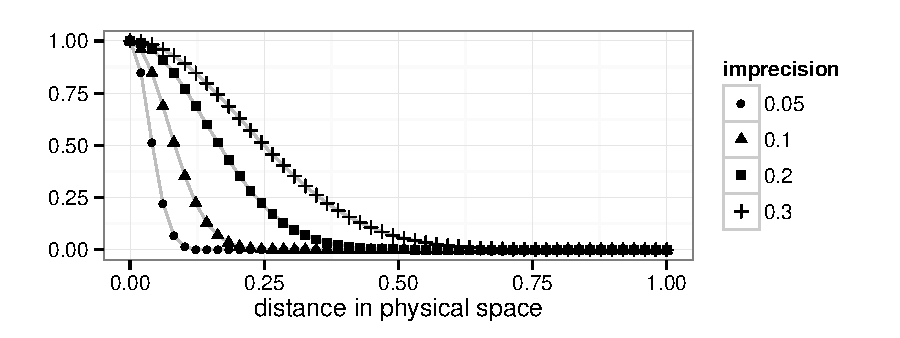
\includegraphics[width=0.7\textwidth]{plots/NosofskySim.pdf}

  \caption{Examples of Nosofsky-similarity for different values of
    imprecision.}
  \label{fig:NosofskySim}
\end{figure}


We further assume that the probability of confusing any two states $\mystate{i}$ and
$\mystate{j}$ is proportional to their perceived similarity and, to keep matters simple, that
observation noise $P_o$ is simply the same as realizational confusability $P_r$ and
that both are governed by the same imprecision parameter $\alpha$:
\begin{align*}
  P_o(\mystate{o} \probbar \mystate{a}) & \propto \similarity(\mystate{o}, \mystate{a} \myts ; \myts
  \imprecision)\,, &   P_r(\mystate{r} \probbar \mystate{i}) & \propto \similarity(\mystate{r}, \mystate{i} \myts ; \myts
  \imprecision) \,.
\end{align*}
For $\imprecision = 0$, we obtain trivial confusion probabilities: everything is reduced to
perfect imitation and the replicator dynamic. For $\imprecision > 0$, any state can be confused
for any other state with some positive probability. For the uninteresting case of
$\imprecision \rightarrow \infty$, confusion is maximal and every state can be perceived or
realized as any other state with probability $\nicefrac{1}{\card{\States}}$.

As for utility, we define it in terms of similarity and introduce another free parameter,
$\toler \ge 0$.  The intention is for this parameter to model the amount of tolerable pragmatic
slack, which should be allowed to vary separately from perceptual imprecision:
\begin{align*}
  \util(\mystate{i}, \mystate{j} \myts ; \myts \toler) =
      \similarity(\mystate{i}, \mystate{j} \myts ; \myts \toler)\,.
\end{align*}
This choice of utility function is governed partly by convenience, but also because we believe it has the right general properties for a communicative payoff function.
Unlike utilities that are, say, linearly or
quadratically decreasing in physical distance
\citep[c.f.][]{JagerMetzger2011:Voronoi-Languag,FrankeJager2010:Vagueness-Signa}, utilities
that are exponentially decreasing in negative quadratic distance can model situations where a
small amount of imprecision in communication is tolerable, whereas similarly small differences
in intolerably far away interpretations matter very little, with a smooth transition between
these regimes \citep[c.f.][]{OConnor2013:The-Evolution-o}.

In order to simplify the analysis, we focus on games with two messages, i.e., we fix $\card{M} = 2$.
In sum, to structure thinking about the behavior of our imprecise imitation dynamic, the system
is governed by three parameters: the number $\ns = \card{T}$ of states in the state space,
imprecision $\imprecision$ and tolerance $\toler$.


\subsection{Simulation set-up}
\label{sec:simulations}

We ran 50 trials of the discrete-time dynamic in (\ref{eq:nRD}), starting with randomly sampled
sender and receiver strategies, for each triplet of independent parameter values:
$\ns \in \set{6, 10, 50, 90}$, $\imprecision \in \set{0, 0.05, 0.1, 0.2, 0.3}$,
$\toler \in \set{0.05, 0.1, 0.2, 0.3}$. Each trial ran for a maximum of 200 update steps. A
trial was considered converged, and thus stopped before the maximum of 200 rounds, if the total
amount of change between strategies before and after an update step was smaller than a suitably
chosen threshold. It is not guaranteed that strategies at halting time had converged to the
eventual attracting state, whether they ran for 200 rounds or not. Our notion of convergence is
therefore only a categorical measure for reaching a certain (well-considered, but eventually
arbitrary) degree of stability. In other words, our notion of ``convergence'' is a measure of
relative speed: is it true that the system reached a state in which evolutionary adaptations
had slowed down almost to a halt before 200 update steps? This is motivated by pragmatic
concerns regarding length of simulation time, but also theoretically justified, because we
hypothesize that confusability of states leads to regularization of evolving strategies, which
would show exactly in an increased speed of evolutionary trajectories towards well-behaved and
regular signaling behavior.


\begin{figure}
  \centering

  \begin{subfigure}[]{0.45\textwidth}
    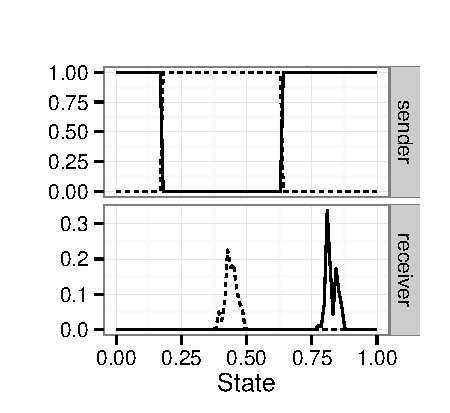
\includegraphics[width=\textwidth]{plots/strat_example_ind3098.pdf}
    \caption{$\ns = 90$, $\toler = 0.1$, $\imprecision = 0$}
    \label{fig:example_stratsA}
  \end{subfigure}
  \hfill
  \begin{subfigure}[]{0.45\textwidth}
    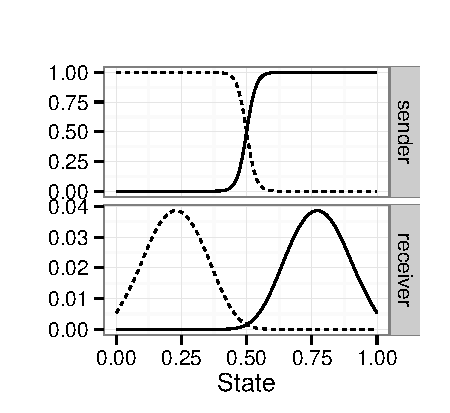
\includegraphics[width=\textwidth]{plots/strat_example_ind1.pdf}
    \caption{$\ns = 90$, $\toler = 0.1$, $\imprecision = 0.05$}
    \label{fig:example_stratsB}
  \end{subfigure}

  % \begin{subfigure}[]{0.45\textwidth}
  %   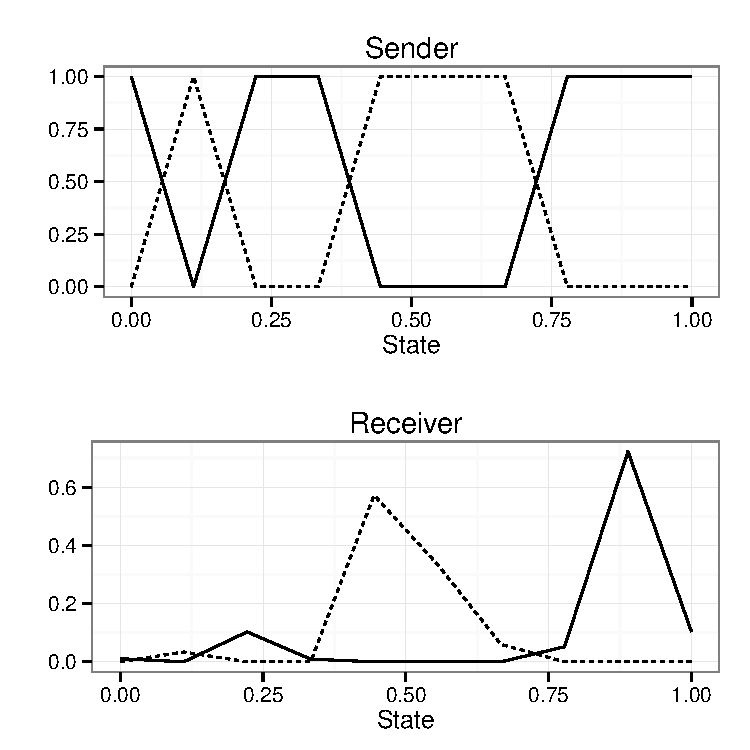
\includegraphics[width=\textwidth]{plots/strat_example_NS-10_tol-005_imp0_ind1001.pdf}
  %   \caption{$\ns = 10$, $\toler = 0.1$, $\imprecision = 0$}
  %   \label{fig:example_stratsC}
  % \end{subfigure}
  % \hfill
  % \begin{subfigure}[]{0.45\textwidth}
  %   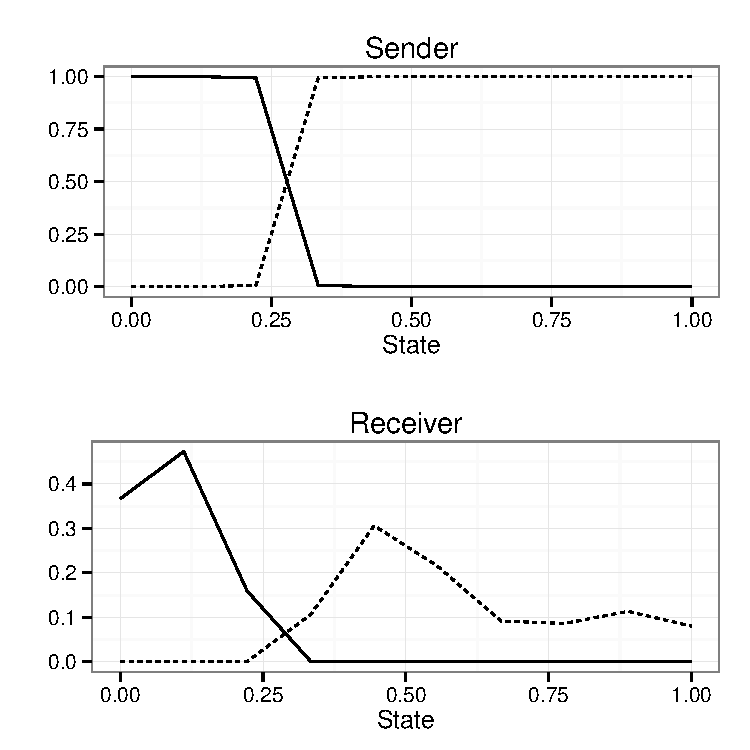
\includegraphics[width=\textwidth]{plots/strat_example_NS-10_tol-005_imp005_ind1201.pdf}
  %   \caption{$\ns = 10$, $\toler = 0.1$, $\imprecision = 0.05$}
  %   \label{fig:example_stratsD}
  % \end{subfigure}


  \caption{Example strategies at stopping time. Each line corresponds to a message and plots, for each state, the probability that the message is used.}
  \label{fig:example_strats}
\end{figure}

Representative examples for resulting strategy pairs are given in
Figure~\ref{fig:example_strats}. Figure~\ref{fig:example_stratsA} shows a strategy pair at
stopping time with 90 states, tolerance $\toler = 0.1$ and imprecision $\imprecision = 0$. Zero
imprecision means that the trial was effectively an application of the standard replicator dynamic. Noteworthily,
the given sender strategy approximates a pure sender strategy that crisply partitions the state
space into non-convex sets. The irregular shape of the receiver strategy suggests that the
pictured strategy pair has not yet reached a stable state. Indeed,
the trial was stopped when reaching the maximum of 200 rounds. In contrast, the outcome of a
trial with identical parameters, except with imprecision $\imprecision = 0.05$, which is shown
in Figure~\ref{fig:example_stratsB}, had converged (in our technical sense) after 99
rounds. The sender strategy shows a smooth blending from one ``category'' to the other, and the
receiver's interpretations are rather extended curves, peaking at a central point in the
relevant ``categories.''

These examples already show two interesting things. Firstly, inclusion of imprecision can lead
to seemingly well-behaved, yet vague strategies in the sense that we are after. The sender
strategy in Figure~\ref{fig:example_stratsB} identifies clear positive and clear negative cases
for each signal, with a smooth transition in-between. The receiver's interpretations of signals
can be seen as smoothed-out prototype regions. Secondly, (sender) strategies can approach
non-convex pure strategies under the replicator dynamic and linger there for vast amounts of
time, possibly indefinitely. We see this in our limited-time simulations (e.g.,
Figure~\ref{fig:example_stratsA}), but this also holds, for some types of utility functions,
for the limiting case. This was first observed by Elliott Wagner, as mentioned by
\citet{OConnor2014-OCOEPC}.  A full analysis of the dynamics of sim-max games is beyond the
scope of this paper, but we will see shortly that diffusion from confusability of states
clearly prevents evolutionary paths that meander for a long time in the vicinity of non-convex
strategies.

\subsection{Measures of interest}
 
To further explore our simulation results, we calculated metrics that aim to numerically
capture how vague, generally well-structured, and communicatively efficient the recorded
strategy pairs were. \emph{Entropy} captures the amount of systematicity or regularity in
signal use. \emph{Convexity} captures whether a behavioral strategy would project onto a convex
pure strategy. \emph{Expected utility} measures the communicative efficiency of evolved
strategy pairs.

\paragraph{Entropy.} This classic information-theoretic notion captures the amount of
uncertainty in a probability distribution. Roughly put, entropy of a signaling strategy
captures inverse distance from a pure strategy. The usual definition of entropy applies
directly to mixed strategies (see Footnote~\ref{fn:mixedStrats}), but provably equivalent
metrics for behavioral strategies are ready to hand:
\begin{align*}
  E(\Sstrat) & = -\sum_{\state \in \States} \sum_{\messg \in \Messgs}
  \Sstrat(\messg \probbar \state) \cdot \log(\Sstrat(\messg \probbar
  \state))\,, &
  E(\Rstrat) & = -\sum_{\messg \in \Messgs} \sum_{\state \in \States}
  \Rstrat(\state \probbar \messg) \cdot \log(\Rstrat(\state \probbar
  \messg)) \,. 
\end{align*}
Values obtained by these definitions have lower bound of zero and an upper bound of,
respectively, $\log(|\Messgs^\States|) = |\States| \cdot \log(|\Messgs|)$ and
$\log(|\States^\Messgs|) = |\Messgs| \cdot \log(|\States|)$. We work with values rescaled to
lie in $[0;1]$ for cross-comparability. The sender strategies in
Figures~\ref{fig:example_stratsA} and \ref{fig:example_stratsB} have entropy $1.19e^{-5}$ and
$0.08$, respectively. The receiver strategies have respective entropies $0.43$ and $0.81$. In
general, we expected that vague languages would have higher entropy than crisp ones and that
increasing imprecision would lead to increased entropy, all else being equal.

\paragraph{Convexity.} At least for sender strategies, which develop faster than receiver
strategies, it also makes sense to define a categorical measure of convexity that compensates
for potential vagueness. To determine whether a sender strategy $\Sstrat$ is convex despite
possibly being vague, we look at the derived pure strategy $\Spure$ for which
$\Spure(\state) = \argmax_{\messg' \in \Messgs} \Sstrat(\state,\messg')$. If that $\Spure$ is
convex, we also count $\Sstrat$ as convex. The sender strategy in
Figure~\ref{fig:example_stratsA} is not convex, while the one in
Figure~\ref{fig:example_stratsB} is.  If confusion of states can regularize signaling
strategies, like we hypothesized, we should see more convexity with increasing imprecision all
else equal.

\paragraph{Expected utility.} We also recorded the expected utility of
a strategy pair:
\begin{align*}
  \EU(\Sstrat,\Rstrat \myts ; \myts \toler) = \sum_{\state \in
    \States} \sum_{\messg \in \Messgs} \sum_{\state' \in \States}
  \Pr(\state) \cdot \Sstrat(\state, \messg) \cdot \Rstrat(\messg,
  \state') \cdot \Util(\state,\state' \myts ; \myts \toler)\,.
\end{align*}
To make direct comparisons across different parameter settings, we
normalize expected utility by the maximal amount of expected utility
obtainable in the relevant game. The strategy pair in
Figure~\ref{fig:example_stratsA} has a normalized expected utility of
$0.99$, the pair in Figure~\ref{fig:example_stratsB} has
$0.95$. Generally, vagueness and imprecision can be expected to
decrease expected utility
\citep[c.f.][]{Lipman2009:Why-is-Language}. The crucial question is
whether communicative success drops unacceptably fast with moderate
levels of vagueness and imprecision.

\subsection{Results}

\begin{figure}[t]
  \centering
  
  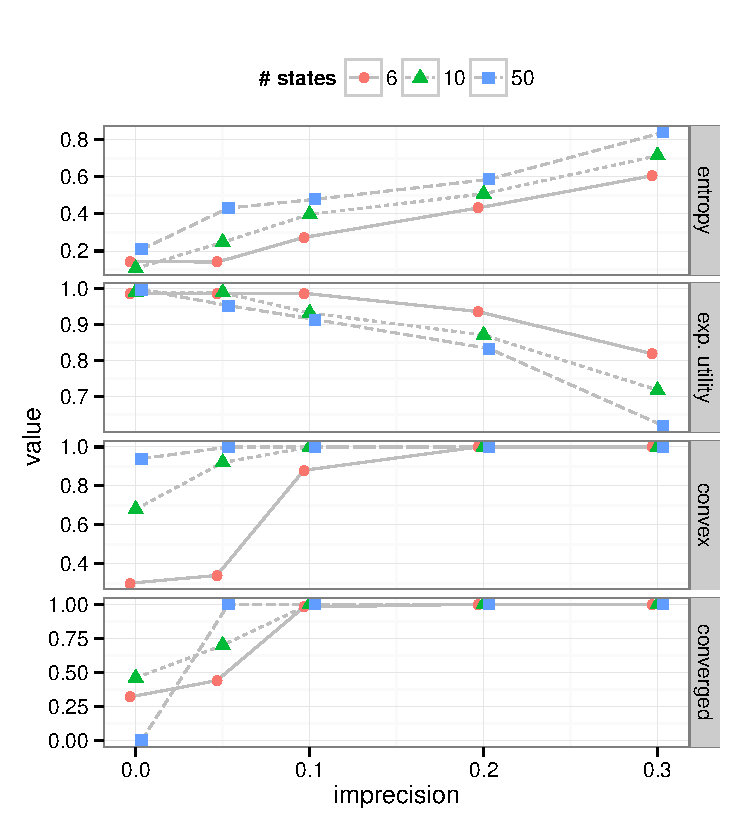
\includegraphics[width=0.75\textwidth]{plots/MeanMetrics3.pdf}

  \caption{Means of gradient and proportions of categorical measures
    for $\toler = 0.1$, $\ns \in \set{6, 10, 50}$, and $\imprecision
    \in \set{0, 0.05, 0.1, 0.2, 0.3}$. The plot shows the average of
    the entropies for the sender and receiver strategy.}
  \label{fig:MeanMetrics}
\end{figure}

Figure~\ref{fig:MeanMetrics} shows plots summarizing a selected part of our findings.  For
perspicuity, we only plot results for one level of tolerance $\beta = 0.1$, and leave out the
case of $n_s = 90$. Still, every qualitative trend mentioned in the following applies to the
whole set of results.

As expected, increasing imprecision leads to higher entropy and lower expected
utility. Importantly, however, imprecision does not necessarily lead to disastrous decline of
communicative success. What is more, in line with our hypothesis that mere imprecision in
imitation behavior can lead to behavior that looks as if agents generalize across similar
stimuli, higher imprecision led to a higher number of outcomes with convex sender
strategies. It also led to higher rates of convergence. In fact, sufficient imprecision always
ensured convergence and convexity. It appears that perceptual imprecision leads to more
vagueness, slightly less communicative efficiency, but more regular, well-behaved languages in
shorter time.

Beyond promoting convexity and convergence, diffusion also has another interesting regularizing
effect on the evolution of signaling. There is very little variation in the recorded metrics
for evolved strategies, at least for higher values of imprecision. On closer inspection, it
turns out that variability in low-imprecision conditions is not only due to non-convergence or
non-convexity. Figure~\ref{fig:MoreExample_strats} gives two more examples of strategy pairs at
stopping time. Both are obtained for the same triple of parameters, both converged before the
maximum number of rounds, and both have convex sender strategies. However, they are not equally
efficient. In fact, the pair in Figure~\ref{fig:example_stratsC} has a normalized expected
utility of $0.99$ while the one in Figure~\ref{fig:example_stratsD} only has $0.89$.


\begin{figure}
  \centering

  \begin{subfigure}[]{0.45\textwidth}
    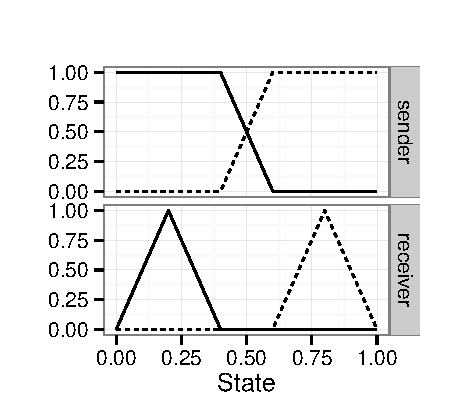
\includegraphics[width=\textwidth]{plots/strat_example_ind21.pdf}
    \caption{$\ns = 6$, $\toler = 0.2$, $\imprecision = 0$}
    \label{fig:example_stratsC}
  \end{subfigure}
  \hfill
  \begin{subfigure}[]{0.45\textwidth}
    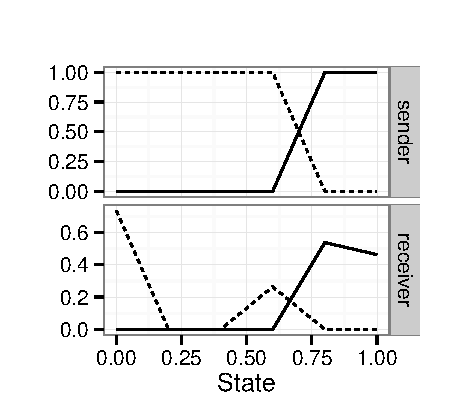
\includegraphics[width=\textwidth]{plots/strat_example_ind23.pdf}
    \caption{$\ns = 6$, $\toler = 0.2$, $\imprecision = 0$}
    \label{fig:example_stratsD}
  \end{subfigure}

  \caption{More example strategies at stopping time of our simulations.}
  \label{fig:MoreExample_strats}
\end{figure}

Interestingly, this type of variability in evolutionary outcomes can
be weeded out by imprecision. To investigate this, we calculated the average
distance between evolved sender strategies within each group of trials
that had identical parameter values. We determined the distance
between strategies $\Sstrat$ and $\Sstrat'$ as the average Hellinger
distance between distributions $\Sstrat(\state)$ and
$\Sstrat'(\state)$ at each choice point $\state$:
\begin{align*}
  \text{HD}(\Sstrat,\Sstrat') & = \frac{1}{{\card{\States} \cdot
     \sqrt{2}}} \cdot  \sum_{\state \in \States} 
 \sqrt{\sum_{\messg \in  \Messgs}
         \left ( \sqrt{\Sstrat(\state,\messg)} -
         \sqrt{\Sstrat'(\state,\messg)} \right )^2 }\,.
\end{align*}
To compensate for the arbitrariness of message use, we set the distance between strategies
$\Sstrat$ and $\Sstrat'$ to be the maximum of $\text{HD}(\Sstrat,\Sstrat')$ and
$\text{HD}(\Sstrat^*,\Sstrat')$ where $\Sstrat^*$ is $\Sstrat$ with reversed message
indices. An example of the \emph{within group distance}, i.e., the average distances between
all sender strategies obtained for the same parameter values, is plotted in
Figure~\ref{fig:GroupMeasuresA} for $\beta = 0.1$ and $n_s = 10$. Despite some quantitative
differences, the general trend is the same for all other parameter settings that we tested:
with increasing imprecision, the resulting sender strategies were much more alike (modulo
swapping of messages). This means that perceptual imprecision can speed up and unify
evolutionary outcomes. It can amplify the emergence of sender strategies that are not only
convex, but also regular in that they induce a vague category split exactly in the middle of
the unit interval.

\begin{figure}
  \centering

  \begin{subfigure}[]{0.45\textwidth}
    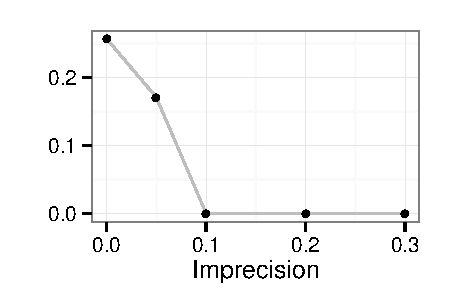
\includegraphics[width=\textwidth]{plots/WithinGroupDistanceConcise.pdf}
    \caption{Within group distance}
    \label{fig:GroupMeasuresA}
  \end{subfigure}
    \hfill
  \begin{subfigure}[]{0.45\textwidth}
    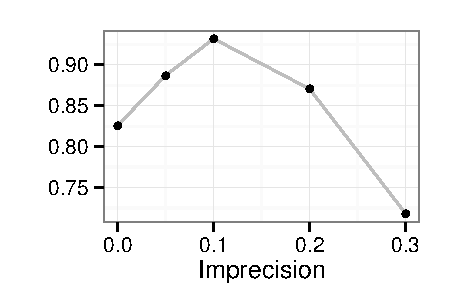
\includegraphics[width=\textwidth]{plots/WithinGroupEUConcise.pdf}
    \caption{Within group expected utility}
    \label{fig:GroupMeasuresB}
  \end{subfigure}

    \caption{Within group measures for all runs with $\toler = 0.1$ and $n_s = 10$.}
  \label{fig:GroupMeasures}
\end{figure}


%%%%%%%%%%%%%%%%%%%%%%%%%%%%%%%%%%%%%%%%%%%%%%%%%%
%%%%%%%%%%%%%%%%%%%%%%%%%%%%%%%%%%%%%%%%%%%%%%%%%%

\section{Discussion}
\label{sec:discussion}

Our imprecise imitation dynamic leads to by-and-large successful signaling behavior, even in
the presence of noise, that shows the hallmarks of vagueness as desired. It also gives rise to
population-level behavior that looks as if agents are generalizing across similar
stimuli. Here, we would like to reflect briefly on some further conceptually relevant points
and compare our approach to related work.

\subsection{Levels of vagueness}
The imprecise imitation dynamic was introduced in Section~\ref{sec:repl-diff-dynam} as tracing
changes in the overall distribution of pure strategies in a population:
$\Sstrat(\messg \probbar \state)$ was said to represent the probability that a randomly sampled
sender would have a strategy that responds with $\messg$ to $\state$ (likewise for the
receiver). This is in line with the standard interpretation of the replicator equation, but we
should consider its philosophical implications. Based on this picture, vagueness in signal use
would seem to be characterized as a strictly population-level phenomenon since it arises in a
signaling system from the inability of individual agents to fully align their (non-vague)
strategies because of imprecision. This is, we believe, a plausible mechanism that can already
explain the existence of vagueness in a language even if we assume that each agent commands a
non-vague idiolect.

We would not, however, want to commit to the idea that vagueness does not exist at the level of
individual agents. True, our derivation of the imprecise imitation dynamic assumed that agents
carry and revise pure strategies. But that was an assumption of convenience, not of
conviction. Moreover, even if individual agents command a non-vague pure strategy, the
realization of that pure strategy, according to our model, is bound to be vague (e.g., the same
agent could signal differently in repeated exposure to the same state). We have used the term
``observation noise'' here, but it may well be that this could equally well be perceived as an
inseparable component of an agent's ``signaling faculty.'' In this sense, then, the model might
be compatible with a picture of agents who have internalized a vague signaling
strategy. It would need to be seen, however, how revision of non-deterministic individual-level
behavior must be spelled out rigorously and whether the resulting population-level dynamic
would be equivalent to our present proposal in all relevant respects.

% Moreover, we believe that the model may be interpreted in yet alternative ways. The
% probability $\Sstrat(\messg \probbar \state)$ merely gives us the likelihood that $\messg$ will
% be used by a sender when observing state $\state$.  Whether the uncertainty represents
% variations in a population of agents playing pure strategies, a single sender using a
% non-deterministic strategy, or even a heterogeneous population of non-deterministic senders, is
% up for interpretation.  The first option supported what we believe to be a plausible motivation
% for the mechanism of imitation of success with imprecision, but other motivations could be
% imagined to better fit an interpretation that includes non-deterministic agents.  We thus
% believe that the model introduced in this paper does not exclude vagueness at the individual
% level, but to explore all possible interpretations would go beyond our current scope.

\subsection{Evolutionary benefits of imprecision}
The inclusion of confusability of similar states has noteworthy effects on the evolving meaning
of signals.  It transpired from our results that imprecision can have further accelerating and,
surprisingly, unifying effects on meaning evolution.  The unifying property of perceptual
imprecision could be considered an evolutionarily beneficial side-effect. A certain degree of
imprecision can lead to higher \emph{within group expected utility}, defined as the average
expected utility that each evolved language scored when playing against an arbitrary other
language obtained for the same parameter values. Figure~\ref{fig:GroupMeasuresB} gives a
representative example. The observation repeats for other parameter values: while imprecision
might decrease the communicative efficiency of individual languages, it increases the
conceptual coherence and communicative success between independently evolving strategies. It is
as if mere confusability of states imposes a regularity constraint on evolving categories.

The phenomenon could potentially not just be a side effect.  Given the benefit of a certain
amount of imprecision we observe when comparing within group expected utility, it would be
interesting to study whether, under certain conditions, this group-level advantage could trump
the individual-level disadvantage of a vague language, and thus actually select for a certain
amount of imprecision.  This could be achieved by letting the imprecision parameter be an
evolving part in the dynamics as well. The idea is for now mostly speculative, but we consider
it an interesting avenue for future research.  There is additional motivation to consider its
potential if we see it in the eyes of multilevel selection theory
\citep{Wilson1994,OGorman2008}.

\subsection{Related work}
\citet{OConnor2013:The-Evolution-o} makes a proposal related to ours based on a version of
reinforcement learning for sim-max games, in which successful play leads to reinforcement of
choice options also for states similar to the ones that actually occurred. This not only leads
to vague signaling of the appropriate kind, but also speeds up learning in such a way that,
especially for sim-max games with higher numbers of states, higher levels of communicative
success are reached in shorter learning periods. Our results complement and extend
\citeauthor{OConnor2013:The-Evolution-o}'s. The most important differences are that we obtain
similar regularizing effects also for cases with low numbers of states and do not assume that
agents have any kind of generalizing capacity in and of themselves, even if that is only
implicit, as in \citeauthor{OConnor2013:The-Evolution-o}'s generalized reinforcement learning.
State confusability has an effect on aggregate signaling behavior that can be described as
generalization without generalizers: the dynamics of imprecise imitation look as if
``conclusions'' about what works for one state are ``carried over'' to similar states. This,
however, is merely an epiphenomenon in the sense that no single agent genuinely generalizes
over stimuli or reasons about what a more systematic signaling strategy would be.


\citet{FrankeJager2010:Vagueness-Signa} suggested a number of ways in which
in\-for\-ma\-tion-processing limitations could lead to vague strategies. The model that is most
clearly related to the present approach uses the notion of a \emph{quantal response}, also
known as a \emph{soft-max response function}
\citep[e.g.][]{Luce1959:Individual-Choi,McFadden1976:Quantal-Choice-,GoereeHolt2008:Quantal-Respons}. The
main difference between this and our present approach is in where stochastic noise is assumed
to reside. In case of a quantal response dynamic, it is the computation of expected utilities;
in case of imprecise imitation, it is perception and realization of similar states. There are
cases, then, where evolving signaling behavior, as predicted by these two approaches, is quite
different. Intuitively speaking, for a case with two messages, the further we venture away from
a prototypical interpretation of either message, the less discriminative a signaling strategy
would be when the source of ``trembles'' is the computation of expected utilities: to wit,
since both ``tall'' and ``short'' are almost equally bad descriptions for a giant, quantal
response dynamics predict that senders would be almost indifferent. Sender behavior that
evolves under confusion of states does not have this puzzling property, because a giant would
not likely be confused for a dwarf. 


%%%%%%%%%%%%%%%%%%%%%%%%%%%%%%%%%%%%%%%%%%%%%%%%%%
%%%%%%%%%%%%%%%%%%%%%%%%%%%%%%%%%%%%%%%%%%%%%%%%%%

\section{Conclusion}
\label{sec:conclusion}

We set out to meet a technical challenge posed by Lipman's problem
\citep{Lipman2009:Why-is-Language}: is there a conceptually sound and mathematically coherent
formal model that shows how vague language can evolve under selective pressure for efficient
communication if agents tend to confuse similar stimuli? To address this, we derived a
generalization of the replicator dynamic from an agent-level process of imprecise
imitation. The resulting population-level dynamic produced signaling behavior that is at the
same time regular and by-and-large communicatively efficient, while also showing the crucial
marks of vagueness. In a sense, the model derives vagueness as a by-product of an arguably
natural limitation on the discriminatory power of signaling agents.  Although inability to
sharply discriminate similar stimuli may lead to vagueness and bring about a (slight) decrease
in communicative efficiency, there may also be an advantage, not of vagueness itself, but of
its reason: systematicity in the confusability of states (which may be a natural by-product of
the perceptual system) supports \emph{as-if}-generalization at the population-level without
having to assume that agents themselves have any generalization power. In this way, the
presented model extends research into the effects of transmission biases on processes of
meaning evolution. While most previous models have focused on inductive biases of language
learners and the regularization that these may effect
\citep[e.g.][]{NowakPlotkin2000:The-Evolution-o,NowakKomarova2001:Evolution-of-Un,KirbyHurford2002:The-Emergence-o,SmithKirby2003:Iterated-Learni,GriffithsKalish2007:Language-Evolut,KirbyGriffith2014:Iterated-Learni},
we have shown here that shared perceptual biases, of which such an effect was not necessarily
expected, can also regularize, facilitate and accelerate the evolution of meaning conventions.


%%%%%%%%%%%%%%%%%%%%%%%%%%%%%%%%%%%%%%%%%%%%%%%%%%
%%%%%%%%%%%%%%%%%%%%%%%%%%%%%%%%%%%%%%%%%%%%%%%%%%

\appendix

\section{Imprecise conditional imitation}
\label{sec:formal-stuff}

The goal of this section is to provide technical details for
Section~\ref{sec:repl-diff-dynam}. We first show, in Section~\ref{sec:cond-imit-succ}, how to
derive the standard replicator dynamic from noise-free imitation of success. Then, in
Section~\ref{sec:imit-succ-with}, we derive the imprecise imitation dynamic by a parallel
chain of arguments.


\subsection{Deriving the replicator dynamic from imitation of success}
\label{sec:cond-imit-succ}

The main idea behind \emph{imitation of success} is that agents imitate the behavior of other
agents at some choice point with a probability that is proportional to the expected utility of
the latter agents' choice. Since the sim-max games that we are looking at here have positive
utilities upper bound by 1, we can identify the switching probability with the expected
utility.

Let's consider sender strategies, as the receiver case is parallel. Call (misleadingly!) the
agent who gets a chance to change behavior ``learner'' and the possibly to-be-imitated agent
``teacher.'' A random learner is drawn from the population and given a chance to change
behavior at choice point $\state$. The probability that our learner plays $\messg$ is
$\Sstrat(\messg \probbar \state)$. The learner observes what a randomly sampled teacher does at
$\state$. That would be $\messg'$ with probability $\Sstrat(\messg' \probbar \state)$. The
learner then starts using $\messg'$ instead of $\messg$ with probability
$\EU(\messg', \state, \Rstrat)$. (Of course, $\messg'$ and $\messg$ could be the same; the
learner could even be the teacher as well, by random sampling.)

If agents get repeated update chances for their choice points, the \emph{expected change} of
frequency of $\messg$-choices at $\state$ becomes:
\begin{align}
  \label{eq:MeanChange}
  \dot{\Sstrat}(\messg \probbar \state) = P(\messg' \rightarrow m, \state) - P(\messg \rightarrow m', \state)\,,
\end{align}
where $P(\messg' \rightarrow m, \state)$ is the ``inflow'' probability that agents switch from
any $\messg'$ to $\messg$ and $P(\messg \rightarrow m', \state)$ is the ``outflow'' probability
that agents switch from $\messg$ to any $\messg'$. Since we are dealing with expectations in a
huge population, these can be spelled out as:
\begin{align*}
  P(\messg' \rightarrow m, \state) & = \sum_{\messg'} \underbrace{\Sstrat(\messg' \probbar
    \state)}_{\text{learner plays $\messg'$}} \cdot
  \underbrace{\Sstrat(\messg \probbar \state)}_{\text{teacher plays $\messg$}} \cdot
  \underbrace{\EU(\messg, \state, \Rstrat)}_{\text{EU teacher choice}} \\
  P(\messg \rightarrow m', \state) & = \sum_{\messg'} \underbrace{\Sstrat(\messg \probbar
    \state)}_{\text{learner plays $\messg$}} \cdot
  \underbrace{\Sstrat(\messg' \probbar \state)}_{\text{teacher plays $\messg'$}} \cdot
  \underbrace{\EU(\messg', \state, \Rstrat)}_{\text{EU teacher choice}}
\end{align*}
From this, we can simplify the expression of expected change in Equation~(\ref{eq:MeanChange})
to:
\begin{align*}
  \dot{\Sstrat}(\messg \probbar \state) & = \Sstrat(\messg \probbar \state) \cdot \EU(\messg,
  \state, \Rstrat) - \Sstrat(\messg \probbar \state) \cdot  \sum_{\messg'}
      \Sstrat(\messg' \probbar \state) \cdot \EU(\messg',\state,\Rstrat) \\
& = \underbrace{\Sstrat(\messg \probbar
    \state)}_{\text{frequency of $\messg$ at $\state$}}  \Big ( \underbrace{\EU(\messg,
  \state, \Rstrat)}_{\text{EU of $\messg$ at $\state$}} -   \underbrace{\sum_{\messg'}
      \Sstrat(\messg' \probbar \state) \cdot \EU(\messg',\state,\Rstrat)}_{\text{average
      EU at choice point $\state$}} \Big )\,.
\end{align*}
This latter formulation is the continuous-time version of the replicator dynamic. We obtain a
discrete-time formulation from it by assuming that discrete update steps are infinitesimally
small, so that:
 \begin{align*}
    \dot{\sigma}(\messg \probbar \state) & = \sigma'(\messg \probbar \state) - \sigma(\messg
    \probbar \state)\\ 
    & = \frac{\Sstrat(\messg \probbar
    \state)  \myts \EU(\messg,\state,\Rstrat)}{\sum_{\messg'}\Sstrat(\messg' \probbar
    \state)  \myts \EU(\messg,\state,\Rstrat)} - \sigma(\messg
      \probbar \state) \\
    & = \frac{\Sstrat(\messg \probbar
    \state)  \myts \EU(\messg,\state,\Rstrat) - \Sstrat(\messg \probbar \state) \sum_{\messg'}\Sstrat(\messg' \probbar
    \state)  \myts \EU(\messg,\state,\Rstrat) }{\sum_{\messg'}\Sstrat(\messg' \probbar
    \state)  \myts \EU(\messg,\state,\Rstrat)}
      \,.
  \end{align*}
By dropping the denominator, which is constant for all $\messg$ for fixed
$\state$, we obtain the above continuous-time formulation.


\subsection{Imitation of success with imprecision}
\label{sec:imit-succ-with}

The above derivation of the replicator dynamic assumes that agents can discriminate choices and
choice points perfectly. Let's dispense with that assumption. With an eye toward sim-max games,
we will assume that states, but not messages, may be confused for one another.\footnote{It is
  relatively straightforward to also incorporate confusability of messages, but this is
  irrelevant to our present purposes.} Confusability of states will affect how agents behave,
how they perceive the behavior of others, and the expected utilities of behavioral
dispositions.

To keep matters simple, let us assume that agents carry pure dispositions to act. Noise can
affect the realization of these strategies. As a sender, every agent maps states to messages:
these are subjectively perceived states, and no longer necessarily also the actually occurring
states. As a receiver, every agent maps messages to state interpretations: these are intended
interpretations that need not always be faithfully realized. This means that behavioral
strategies $\Sstrat$ and $\Rstrat$ represent the average proportions of \emph{actual}
behavioral dispositions in the population, the realization and observation of which can be
distorted by agents' confusion of similar states.

If $\mystate{a}$ is the actual state, let $P_o(\mystate{o} \probbar \mystate{a})$ be the
probability that a given agent observes state $\mystate{o}$. Similarly, if a given receiver
intends to select interpretation $\mystate{i}$, let $P_r(\mystate{r} \probbar \mystate{i})$ be
the probability with which state $\mystate{r}$ is realized. A single round of play of a sim-max
game is then governed by five pieces of stochastic information, where previously there were
only three (see Figures~\ref{fig:sim-max-illustration} and
\ref{fig:imprecise-sim-max-illustration}). 

Expected utilities of choices at choice points should likewise take into account that actual states
need not be observed states, and intended interpretations need not be realized
interpretations. First, note that
\begin{align*}
  P_{\overline{o}}(\mystate{a} \probbar \mystate{o}) \propto P_a(\mystate{a}) P_o(\mystate{o}
    \probbar \mystate{a})
\end{align*}
is the probability that $\mystate{a}$ is actual if $\mystate{o}$ is observed by an agent. The
probability that a random sender produces $\messg$ when the actual state is $\mystate{a}$ is:
\begin{align*}
  P_{\Sstrat}(\messg \probbar \mystate{a}) = \sum_{\mystate{o}} P_o(\mystate{o} \probbar
  \mystate{a}) \Sstrat(\messg \probbar \mystate{o})\,. 
\end{align*}
The probability that the actual state is $\mystate{a}$ if a random sender produced $\messg$ is:
\begin{align*}
  P_{\overline{\Sstrat}}(\mystate{a} \probbar \messg) \propto P_a(\mystate{a})
  P_{\Sstrat}(\messg \probbar \mystate{a})\,. 
\end{align*}
The probability that $\mystate{r}$ is realized by a random receiver in response to
message $\messg$ is:
\begin{align*}
  P_{\Rstrat}(\mystate{r} \probbar \messg) = \sum_{\mystate{i}} P_r(\mystate{r} \ \probbar
  \mystate{i}) \Rstrat(\mystate{i} \probbar \messg)\,.
\end{align*}
This lets us capture the expected utilities for observed states (sender) and intended
interpretations (receiver) by taking into consideration what the likely actual states and
realized interpretations will be:
\begin{align*}
  \EU(\messg , \mystate{o}, \Rstrat) & = \sum_{\mystate{a}} P_{\overline{o}}(\mystate{a}
  \probbar \mystate{o}) \sum_{\mystate{r}} P_\Rstrat(\mystate{r} \probbar
  \messg) \utils(\mystate{a}, \mystate{r})\,, \\
  \EU(\mystate{i}, \messg, \Sstrat) & = \sum_{\mystate{a}} P_{\overline{\Sstrat}}(\mystate{a}
  \probbar \messg) \sum_{\mystate{r}} P_{r}(\mystate{r} \probbar \mystate{i})
  \utils(\mystate{a}, \mystate{r})\,.
\end{align*}
If the conditional probabilities $P_o$ and $P_r$ are trivial, i.e., assign probability 0 to the
confusability of non-identical states, above definitions reduce to the
previous definitions of expected utilities. This also legitimates the overload of notation.


Presence of potential imprecision in the form of non-trivial $P_o$ and $P_r$ will also affect
the dynamic that ensues from imitation of successes. Since imprecision works slightly
differently on senders and receivers (the former confuse choice points, the latter confuse
choices), we need to look separately at each case.

As before, suppose that senders receive a chance to change their behavior independently for a
given choice point. In the present case, this would be a chance to change how to respond to a
subjectively perceived state $\mystate{o}$, which need not be the actual one. We must then
consult the probability $P_o(\messg \probbar \mystate{o})$ that, given that the learner
observed $\mystate{o}$, he will simultaneously observe a randomly sampled teacher play
$\messg$. This is (with $P_{\overline{o}}$ and $P_{\Sstrat}$ as defined above):
\begin{align*}
  P_o(\messg \probbar \mystate{o}) = \sum_{\mystate{a}} P_{\overline{o}}(\mystate{a}
  \probbar \mystate{o}) \myts P_{\Sstrat}(\messg \probbar \mystate{a})\,.
\end{align*}
The ``inflow'' and ``outflow'' probabilities $P(\messg' \rightarrow \messg, \state)$ and
$P(\messg' \rightarrow \messg, \state)$ that a randomly sampled learner switches from any
$\messg'$ to $\messg$ or from $\messg$ to any $\messg'$ in subjectively perceived state
$\mystate{o}$ are therefore:
\begin{align*}
  P(\messg' \rightarrow \messg, \mystate{o}) & = \sum_{\messg'} \underbrace{\Sstrat(\messg' \probbar
    \mystate{o})}_{\text{learner plays $\messg'$ at $\mystate{o}$}} \cdot
  \underbrace{P_{o}(\messg \probbar \mystate{o})}_{\text{observe teacher play $\messg$}} \cdot
  \underbrace{\EU(\messg, \mystate{o}, \Rstrat)}_{\text{EU teacher choice in learner's view}}
  \\
  P(\messg \rightarrow \messg', \mystate{o}) & = \sum_{\messg'} \underbrace{\Sstrat(\messg \probbar
    \mystate{o})}_{\text{learner plays $\messg$ at $\mystate{o}$}} \cdot
  \underbrace{P_{o}(\messg' \probbar \mystate{o})}_{\text{observe teacher play $\messg'$}} \cdot
  \underbrace{\EU(\messg', \mystate{o}, \Rstrat)}_{\text{EU teacher choice in learner's view}}
\end{align*}
The mean change to the proportion of $\messg$ choices at state $\state$ are then:
\begin{align}
  \label{eq:nRDSender}
  \dot{\Sstrat}(\messg \probbar \mystate{o}) & = P(\messg' \rightarrow m, \mystate{o}) - P(\messg
  \rightarrow m', \mystate{o}) \nonumber \\
  & = \sum_{\messg'} \Sstrat(\messg' \probbar \mystate{o}) \myts P_o(\messg \probbar
  \mystate{o}) \myts \EU(\messg, \mystate{o}, \Rstrat) - \sum_{\messg'} \Sstrat(\messg \probbar \mystate{o}) \myts
  P_o(\messg' \probbar \mystate{o}) \myts \EU(\messg', \mystate{o}, \Rstrat) \nonumber \\
  & = P_o(\messg \probbar \mystate{o}) \myts \EU(\messg, \mystate{o}, \Rstrat) - \Sstrat(\messg \probbar \mystate{o}) \myts \sum_{\messg'} P_o(\messg' \probbar \mystate{o}) \myts \EU(\messg', \mystate{o}, \Rstrat)\,.
\end{align}


The case of the receiver is mostly analogous. Presented with an update opportunity for choice
point $\messg$, a learner will observe a random teacher choose interpretation $\mystate{o}$
with probability:\footnote{We assume that the noise $P_o(\mystate{o} \probbar \mystate{a})$
  that applies to the sender's observations also applies to the receiver's observations when
  trying to imitate other agents' strategies. We could easily make the model more complex and
  introduce another measure of noise for state confusability during receiver attempts to
  imitate. We refrain from it here, because we see no immediate theoretical gain.}
\begin{align*}
  P_o(\mystate{o} \probbar \messg) = \sum_{\mystate{r}} P_o(\mystate{o} \probbar \mystate{r})
  \myts P_{\Rstrat}(\mystate{r} \probbar \messg) % = \sum_{\mystate{r}} P_o(\mystate{o} \probbar \mystate{r})
  % \myts \sum_{\mystate{i}} P_r(\mystate{r} \ \probbar
  % \mystate{i}) \myts \Rstrat(\mystate{i} \probbar \messg)
  \,.
\end{align*}
% The probability $P(\state' \rightarrow \state, \messg)$ that a randomly sampled learner switches
% from using $\state'$ to $\state$ in response to $\messg$ is therefore:
% \begin{align*}
%   P(\state' \rightarrow \state, \messg) = \sum_{\state'} \underbrace{\Rstrat(\state' \probbar
%     \messg)}_{\text{learner plays $\state'$}} \cdot
%   \underbrace{P_{o}(\state \probbar \messg)}_{\text{observe teacher play $\state$}} \cdot
%   \underbrace{\EU(\state, \messg, \Rstrat)}_{\text{EU teacher choice}}
% \end{align*}
Parallel to the sender case, this gives rise to:
\begin{align}
  \label{eq:nRDReceiver}
  \dot{\Rstrat}(\state \probbar \messg) & = \sum_{\state'} \Rstrat(\state' \probbar \messg)
  \myts P_o(\state \probbar \messg) \myts \EU(\state, \messg, \Sstrat) - \sum_{\state'}
  \Rstrat(\state \probbar \messg) \myts
  P_o(\state' \probbar \messg) \myts \EU(\state', \messg, \Sstrat) \nonumber \\
  & = P_o(\state \probbar \messg) \myts \EU(\state, \messg, \Sstrat) - \Rstrat(\state \probbar
  \messg) \myts \sum_{\state'}
  P_o(\state' \probbar \messg) \myts \EU(\state', \messg, \Sstrat) 
\end{align}

The continuous-time formulations in Equations~(\ref{eq:nRDSender}) and (\ref{eq:nRDReceiver})
have elegant and practical discrete-time solutions in:
\begin{align*}
  \Sstrat'(\messg \probbar \state) & \propto P_o(\messg \probbar \state) \myts \EU(\messg,
  \state, \Rstrat)\,, & \Rstrat'(\state \probbar \messg) & \propto P_o(\state \probbar \messg)
  \myts \EU(\state, \messg, \Sstrat)\,,
\end{align*}
which is the discrete-time formulation of the imprecise imitation dynamic given in
Equation~(\ref{eq:nRD}). To see how the discrete-time formulation gives rise to the
continuous-time formulations above, let's assume that update steps are infinitesimally small,
so that, for the sender case:
\begin{align*}
  \dot{\sigma}(\messg \probbar \state) & = \sigma'(\messg \probbar \state) - \sigma(\messg
  \probbar \state)\\
  &= \frac{P_o(\messg \probbar \state) \myts \EU(\messg, \state, \Rstrat) - \Sstrat(\messg
    \probbar \state) \sum_{\messg'} P_o(\messg' \probbar \state) \myts \EU(\messg', \state,
    \Rstrat) }{ \sum_{\messg'} P_o(\messg' \probbar \state) \myts \EU(\messg', \state,
    \Rstrat)}\,.
\end{align*}
As before, we drop the denominator, which is constant for all $\messg$ for fixed $\state$, and
obtain the above continuous-time formulation.

%%%%%%%%%%%%%%%%%%%%%%%%%%%%%%%%%%%%%%%%%%%%%%%%%%
%%%%%%%%%%%%%%%%%%%%%%%%%%%%%%%%%%%%%%%%%%%%%%%%%%

\printbibliography[heading=bibintoc]

\end{document}
